\chapter{Vivo ou não vivo?}\label{ch:g1:living-or-not}

Um caracol desliza devagar pelo caminho molhado. Do lado dele está
uma pedrinha cinza, do mesmo tamanho e igualmente redonda. O caracol
e a pedrinha estão debaixo da mesma chuva --- mas um dos dois está
vivo e o outro não. Como é que a gente sabe? Essa é a primeira
pergunta da \omterm{def:g1:living-or-not:living}{biologia}, a ciência dos \omterm{def:g1:living-or-not:living}{seres vivos}.

\section{O que os seres vivos fazem}

\begin{definition}[Ser vivo]\label{def:g1:living-or-not:living}
Um \emph{ser vivo}\index{ser vivo} é algo que está
\emph{vivo}\index{vivo}: ele nasce, se alimenta, cresce, pode ter
filhotes e um dia morre. Os animais e as plantas são seres vivos. A
biologia\index{biologia} é a ciência que estuda os seres vivos.
\end{definition}

\begin{example}[O caracol e a pedrinha]\label{ex:g1:living-or-not:snail}
O caracol nasceu de um ovinho. Ele come folhas de alface. Ele cresce
--- e a concha cresce junto com ele. Pode haver filhotes de caracol.
Então o caracol é um \omterm{def:g1:living-or-not:living}{ser vivo}. A pedrinha não come nada, não cresce
nem um pouquinho e nunca tem pedrinhas filhotes: a pedrinha não é viva.
\end{example}


\begin{omfigure}
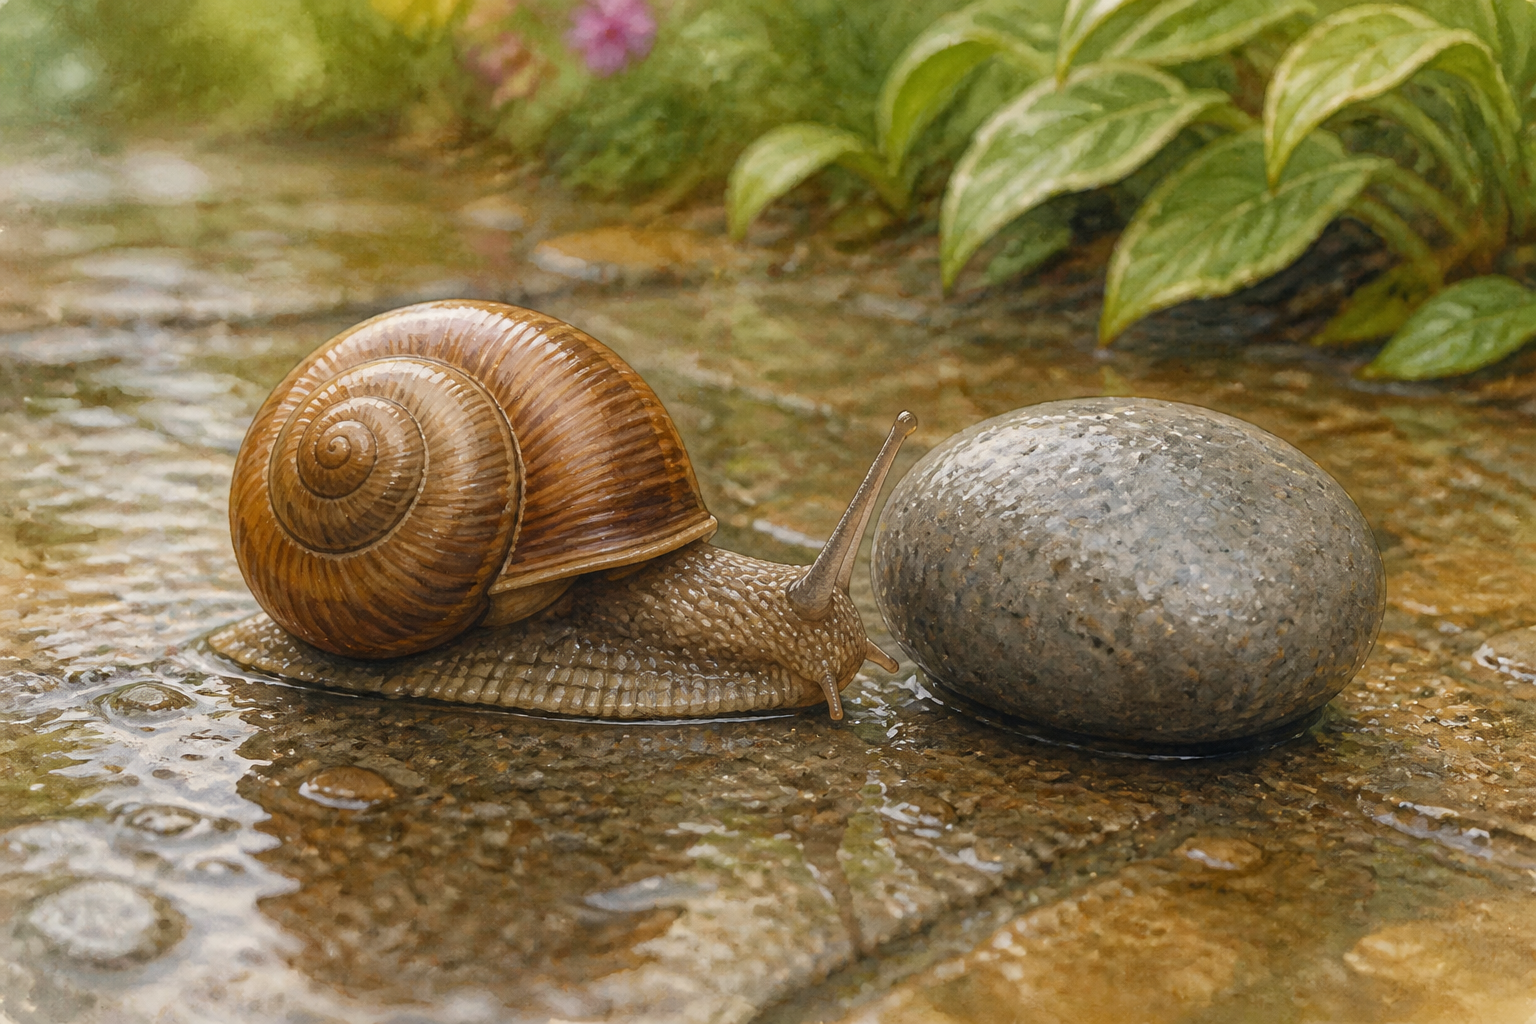
\includegraphics[width=0.62\linewidth]{images/book1/ai/g1-living-snail.png}

{\small Os dois vizinhos deste capítulo em pessoa: um deles está
indo devagar para algum lugar --- e não é a pedrinha.}
\end{omfigure}

\begin{proposition}[Os sinais da vida]\label{prop:g1:living-or-not:signs}
Um \omterm{def:g1:living-or-not:living}{ser vivo} mostra estes sinais:
\begin{enumerate}
  \item ele \emph{nasce}\index{nascer};
  \item ele \emph{se alimenta}\index{alimentar-se} --- come ou fabrica
        a própria comida, como as plantas fazem com a luz;
  \item ele \emph{cresce}\index{crescer};
  \item ele pode ter filhotes --- novos \omterm{def:g1:living-or-not:living}{seres vivos} parecidos com ele;
  \item ele \emph{morre}\index{morrer} um dia.
\end{enumerate}
Uma coisa que não mostra nenhum desses sinais não é viva.
\end{proposition}
\admitted

\begin{remark}[Todos os sinais contam]\label{rem:g1:living-or-not:allsigns}
Um sinal sozinho não basta. Um carro ``bebe'' combustível, e um
pingente de gelo fica mais comprido no frio --- mas o carro foi
construído, não nasceu, e o gelo não tem gelinhos filhotes. Para
estar vivo, algo precisa mostrar os sinais da vida \emph{juntos}:
nascer, se alimentar, crescer, fazer novos \omterm{def:g1:living-or-not:living}{seres vivos}, morrer.
\end{remark}

\section{Vivo, não vivo, nunca vivo}

\begin{definition}[Coisa não viva]\label{def:g1:living-or-not:nonliving}
Uma \emph{coisa não viva}\index{coisa não viva} é algo que não está
vivo. Há dois tipos:
\begin{itemize}
  \item coisas que \emph{nunca estiveram vivas}\index{nunca esteve
        vivo}: uma pedrinha, a água, o vento, uma bicicleta;
  \item coisas que \emph{não estão mais vivas}\index{não está mais
        vivo} ou que \emph{vêm de} \omterm{def:g1:living-or-not:living}{seres vivos}: uma folha seca no
        chão, uma mesa de madeira, um casaco de lã.
\end{itemize}
\end{definition}

\begin{example}[A mesa de madeira]\label{ex:g1:living-or-not:table}
Uma mesa de madeira não se alimenta e não cresce: ela não é viva.
Mas a madeira dela já foi viva: vem de uma árvore que nasceu de uma
semente, cresceu por muitos anos e foi cortada. A mesa é uma \omterm{def:g1:living-or-not:nonliving}{coisa
não viva} --- e vem de um \omterm{def:g1:living-or-not:living}{ser vivo}.
\end{example}

\begin{example}[E um robô?]\label{ex:g1:living-or-not:robot}
Um robô de brinquedo anda, faz barulho e a luzinha dele pisca como
um olhinho. Ele está vivo? Confira os sinais: ele foi montado numa
fábrica, não nasceu; a pilha não é comida que o faça crescer; ele
nunca vai ter robôs filhotes. O robô se mexe, mas não é vivo.
\end{example}

\begin{omfigure}
\begin{tikzpicture}
  % three sorting boxes
  \draw[thick, omDef, fill=omDef!6] (0,0) rectangle (3.9,2.6);
  \draw[thick, omProp, fill=omProp!6] (4.3,0) rectangle (8.2,2.6);
  \draw[thick, omExo, fill=omExo!6] (8.6,0) rectangle (12.5,2.6);
  \node[font=\small\bfseries, omDef] at (1.95,2.25) {vivo};
  \node[font=\small\bfseries, omProp] at (6.25,2.25) {já foi vivo};
  \node[font=\small\bfseries, omExo] at (10.55,2.25) {nunca foi vivo};
  \node[font=\small, align=center, text width=3.6cm] at (1.95,1.1)
    {um caracol\\ uma margarida\\ você!};
  \node[font=\small, align=center, text width=3.6cm] at (6.25,1.1)
    {uma folha seca\\ uma colher de pau\\ uma pena no caminho};
  \node[font=\small, align=center, text width=3.6cm] at (10.55,1.1)
    {uma pedrinha\\ uma poça\\ uma bolinha de gude};
\end{tikzpicture}

{\small Três caixas para separar o mundo: vivo, não é mais vivo,
nunca foi vivo.}
\end{omfigure}

\begin{method}[Como decidir: vivo ou não?]\label{met:g1:living-or-not:decide}
Faça as perguntas da vida, uma de cada vez:
\begin{enumerate}
  \item Nasceu? Se alimenta? Cresce?
  \item Pode ter filhotes? Vai morrer um dia?
  \item Se as respostas forem sim: é vivo.
  \item Se as respostas forem não, faça mais uma pergunta: será que
        \emph{vem de} algo vivo, como a madeira vem da árvore?
\end{enumerate}
\end{method}

\begin{remark}[As sementes parecem dormindo]\label{rem:g1:living-or-not:seed}
Um feijão seco dentro do pacote parece tão paradinho quanto uma
pedrinha. Mas ponha ele num algodão molhado e, em poucos dias,
aparece uma raizinha: a semente estava viva o tempo todo, esperando.
Os \omterm{def:g1:living-or-not:living}{seres vivos} lentos e quietos são fáceis de confundir com \omterm{def:g1:living-or-not:nonliving}{coisas
não vivas} --- as perguntas da vida ajudam a olhar melhor.
\end{remark}

\section{Exercícios}

\begin{exercise}[$\star$]\label{exo:g1:living-or-not:1}
Diga os cinco sinais da vida. Quais deles você consegue ver um
gatinho fazendo hoje?
\end{exercise}

\begin{exercise}[$\star$]\label{exo:g1:living-or-not:2}
Vivo ou não vivo? (a) uma borboleta; (b) uma bicicleta; (c) uma
margarida; (d) uma nuvem.
\end{exercise}

\begin{exercise}[$\star$]\label{exo:g1:living-or-not:3}
Uma folha seca está caída no caminho. Ela está viva agora? Já esteve
viva alguma vez? De onde ela veio?
\end{exercise}

\begin{exercise}[$\star$]\label{exo:g1:living-or-not:4}
O Tomás diz: ``O rio está vivo --- olha, ele se mexe e faz
barulho!'' Use as perguntas do \cref{met:g1:living-or-not:decide}
para responder a ele com jeitinho.
\end{exercise}

\begin{exercise}[$\star$]\label{exo:g1:living-or-not:5}
Separe nas três caixas da figura --- vivo, já foi vivo, nunca foi
vivo: uma aranha, uma meia de lã, uma gota de chuva, uma maçã na
árvore, uma pinha caída.
\end{exercise}

\begin{exercise}[$\star$]\label{exo:g1:living-or-not:6}
A chama de uma vela ``come'' a cera, fica mais alta e morre quando
você assopra. A chama é um \omterm{def:g1:living-or-not:living}{ser vivo}? Qual pergunta da vida diz que
não?
\end{exercise}

\begin{exercise}[$\star$]\label{exo:g1:living-or-not:7}
Diga duas coisas do seu quarto que vêm de \omterm{def:g1:living-or-not:living}{seres vivos}, como a mesa
de madeira do \cref{ex:g1:living-or-not:table}. Diga de que \omterm{def:g1:living-or-not:living}{ser vivo}
cada uma delas vem.
\end{exercise}

\begin{exercise}[$\star$]\label{exo:g1:living-or-not:8}
Faça a experiência: ponha um feijão seco num algodão molhado perto
da janela, e uma pedrinha em outro algodão molhado do lado. Olhe
todo dia durante uma semana. Qual dos dois muda? O que isso mostra?
\end{exercise}

\begin{exercise}[$\star\star$]\label{exo:g1:living-or-not:9}
Um robô de brinquedo e um caracol atravessam o chão. Dê duas
perguntas da vida em que as respostas dos dois são diferentes.
\end{exercise}

\begin{exercise}[$\star\star$]\label{exo:g1:living-or-not:10}
Os cogumelos não correm como os animais e não são verdes como quase
todas as plantas. Com os sinais da \cref{prop:g1:living-or-not:signs},
explique por que um cogumelo é mesmo um \omterm{def:g1:living-or-not:living}{ser vivo}.
\end{exercise}
